% F092｜高中数学常用数值表｜02_explanation.tex
% 继承上传模板的 LaTeX 环境；当前条目的内容独立编写。
\clearpage
\begin{explanationbox}
\textbf{\textcolor{CExplanation}{根号常用值：二、三、五是基石}}
\par\medskip
\begin{center}
% F092｜cards 原创简明教学示意图
\begin{tikzpicture}[>=stealth,scale=.92]
\node[draw,rounded corners,fill=teal!9,minimum width=2.7cm,minimum height=1.2cm] at (0,0){$\sqrt2\approx1.414$};
\node[draw,rounded corners,fill=orange!9,minimum width=2.7cm,minimum height=1.2cm] at (3.1,0){$\ln2\approx0.693$};
\node[draw,rounded corners,fill=teal!9,minimum width=2.7cm,minimum height=1.2cm] at (6.2,0){$e\approx2.718$};
\node at (3.2,-1.0){\small 先记少数基准数，其余借公式推导};
\end{tikzpicture}

\end{center}
\medskip
\[\sqrt{2}\approx1.414,\quad \sqrt{3}\approx1.732,\quad \sqrt{5}\approx2.236,\quad \sqrt{6}\approx2.449,\quad \sqrt{7}\approx2.646,\quad \sqrt{8}\approx2.828,\quad \sqrt{10}\approx3.162\]另有 $\sqrt\pi\approx1.772$。不是每项都要死记，例如 $\sqrt6=\sqrt2\sqrt3$、$\sqrt8=2\sqrt2$、$\sqrt{10}=\sqrt2\sqrt5$。
\end{explanationbox}
\clearpage
\begin{explanationbox}
\textbf{\textcolor{CExplanation}{对数：以e为底的ln与以10为底的lg}}
\par\medskip
\begin{center}
% F092｜derive 原创简明教学示意图
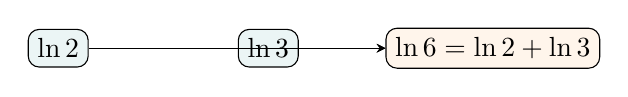
\begin{tikzpicture}[>=stealth,scale=.92]
\node[draw,rounded corners,fill=teal!8] (a) at (0,0){$\ln2$};
\node[draw,rounded corners,fill=teal!8] (b) at (2.9,0){$\ln3$};
\node[draw,rounded corners,fill=orange!8] (c) at (6,0){$\ln6=\ln2+\ln3$};
\draw[->] (a)--(c);\draw[->] (b)--(c);
\end{tikzpicture}

\end{center}
\medskip
\[\begin{array}{c|c|c}
x & \ln x & \lg x\\\hline
2 & 0.693 & 0.301\\
3 & 1.099 & 0.477\\
4 & 1.386 & 0.602\\
5 & 1.609 & 0.699\\
6 & 1.792 & 0.778\\
7 & 1.946 & 0.845\\
8 & 2.079 & 0.903\\
9 & 2.197 & 0.954\\
10 & 2.303 & 1.000\\\end{array}\]其中 $\ln4=2\ln2$、$\ln6=\ln2+\ln3$、$\lg5=1-\lg2$。若从已经四舍五入的数推导，末位结果可能偏差。
\end{explanationbox}
\clearpage
\begin{explanationbox}
\textbf{\textcolor{CExplanation}{指数、圆周率及其组合}}
\par\medskip
\begin{center}
% F092｜cards 原创简明教学示意图
\begin{tikzpicture}[>=stealth,scale=.92]
\node[draw,rounded corners,fill=teal!9,minimum width=2.7cm,minimum height=1.2cm] at (0,0){$\sqrt2\approx1.414$};
\node[draw,rounded corners,fill=orange!9,minimum width=2.7cm,minimum height=1.2cm] at (3.1,0){$\ln2\approx0.693$};
\node[draw,rounded corners,fill=teal!9,minimum width=2.7cm,minimum height=1.2cm] at (6.2,0){$e\approx2.718$};
\node at (3.2,-1.0){\small 先记少数基准数，其余借公式推导};
\end{tikzpicture}

\end{center}
\medskip
\[\begin{aligned}e&\approx2.718, &1/e&\approx0.368, &\sqrt e&\approx1.649,\\ e^2&\approx7.389,&1/e^2&\approx0.135, &\pi^2&\approx9.870,\\ e^\pi&\approx23.141,&e^e&\approx15.154,&\pi^\pi&\approx36.462,\\ \pi^e&\approx22.459,&1/\pi&\approx0.318,&\sqrt\pi&\approx1.772.\end{aligned}\]
\end{explanationbox}
\clearpage
\begin{explanationbox}
\textbf{\textcolor{CExplanation}{平方数、立方数}}
\par\medskip
\begin{center}
% F092｜square 原创简明教学示意图
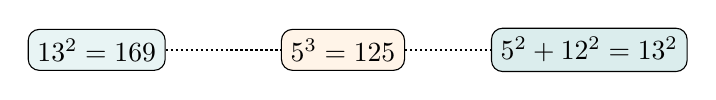
\begin{tikzpicture}[>=stealth,scale=.92]
\node[draw,rounded corners,fill=teal!9] (a) at (0,0){$13^2=169$};
\node[draw,rounded corners,fill=orange!9] (b) at (3.4,0){$5^3=125$};
\node[draw,rounded corners,fill=teal!14] (c) at (6.8,0){$5^2+12^2=13^2$};
\draw[densely dotted,thick] (a)--(b);\draw[densely dotted,thick] (b)--(c);
\end{tikzpicture}

\end{center}
\medskip
\textbf{11 到 30 的平方：}\[\begin{array}{c|c|c|c|c|c}
n & 11 & 12 & 13 & 14 & 15\\\hline
n^2 & 121 & 144 & 169 & 196 & 225\\\end{array}\]
\[\begin{array}{c|c|c|c|c|c}
n & 16 & 17 & 18 & 19 & 20\\\hline
n^2 & 256 & 289 & 324 & 361 & 400\\\end{array}\]
\[\begin{array}{c|c|c|c|c|c}
n & 21 & 22 & 23 & 24 & 25\\\hline
n^2 & 441 & 484 & 529 & 576 & 625\\\end{array}\]
\[\begin{array}{c|c|c|c|c|c}
n & 26 & 27 & 28 & 29 & 30\\\hline
n^2 & 676 & 729 & 784 & 841 & 900\\\end{array}\]\textbf{1 到 10 的立方：}\[\begin{array}{c|c|c|c|c|c}
n & 1 & 2 & 3 & 4 & 5\\\hline
n^3 & 1 & 8 & 27 & 64 & 125\\\end{array}\]
\[\begin{array}{c|c|c|c|c|c}
n & 6 & 7 & 8 & 9 & 10\\\hline
n^3 & 216 & 343 & 512 & 729 & 1000\\\end{array}\]例如 $18^2=324$，不能误记成 $364$。
\end{explanationbox}
\clearpage
\begin{explanationbox}
\textbf{\textcolor{CExplanation}{质数、常用勾股数组}}
\par\medskip
\begin{center}
% F092｜square 原创简明教学示意图
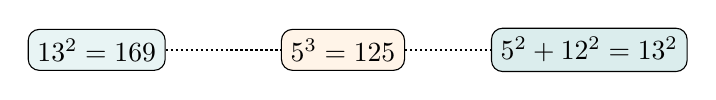
\begin{tikzpicture}[>=stealth,scale=.92]
\node[draw,rounded corners,fill=teal!9] (a) at (0,0){$13^2=169$};
\node[draw,rounded corners,fill=orange!9] (b) at (3.4,0){$5^3=125$};
\node[draw,rounded corners,fill=teal!14] (c) at (6.8,0){$5^2+12^2=13^2$};
\draw[densely dotted,thick] (a)--(b);\draw[densely dotted,thick] (b)--(c);
\end{tikzpicture}

\end{center}
\medskip
\textbf{100以内质数（25个）：} $2,\ 3,\ 5,\ 7,\ 11,\ 13,\ 17,\ 19,\ 23,\ 29,\ 31,\ 37,\ 41,\ 43,\ 47,\ 53,\ 59,\ 61,\ 67,\ 71,\ 73,\ 79,\ 83,\ 89,\ 97$。\par\textbf{常见勾股数组：}$(3,4,5)$、$(5,12,13)$、$(6,8,10)$、$(7,24,25)$、$(8,15,17)$、$(9,12,15)$、$(9,40,41)$、$(20,21,29)$。勾股数构造及穷举分别见 F089、F090。
\end{explanationbox}
